\newpage
\section{Planning of a business intelligence process for a mining data center} \label{toc:planungeinesbiprozessesfuereinminingrechenzentrum}

The following chapter evaluates whether an \ac{BI} process is operationally feasible under the conditions developed in the previous chapter.
For this examination exist among other things two approaches, which are described in the publication
"Business Intelligence Stategy" by John Boyer et al:\footcite[Cf.][p. 102]{boyer2010business}

\begin{itemize}
    \item \textbf{Stakeholder analysis: } In chapter \ref{toc:stakeholderanalyse} the stakeholders of the concerned
    \ac{BI} Process are identified. This makes it possible to identify technological approaches to realization
    and to analyze whether this process will have sufficient support within the company. This support
    depends primarily on how many stakeholders benefit from the added value of a \ac{BI} process.
    Based on this, in chapter \ref{toc:datenpraesentation}
    identifies the appropriate forms of data presentation.\footcite[Cf.][p. 102]{boyer2010business}
    \item \textbf{Technological environment:}The technological environment within the business is analyzed.
    This allows components to be identified that already exist and only need to be integrated.\footcite[Cf.][p. 102]{boyer2010business} Additionally
    the argumentation from chapter \ref{toc:ansatzmoeglichkeitenfuerbusinessintelligence} can be extended or supported with it.
    As technological basis for the realization the Google Cloud is considered, since this is used within the
    Genesis Group is strongly used.
\end{itemize}

To obtain meaningful results on these two points, a small case study is designed in chap.
\ref{toc:fallstudiendesign} is designed so that operational feasibility can be tested. Towards the end of the chapter, the
results from this study are briefly summarized and evaluated. A critical evaluation of the entire argumentation takes place
in the conclusion of this thesis.

\subsection{Case study design and methodology} \label{toc:fallstudiendesign}

In this part, the basic structure of the case study is described. For the design of the case study the approach of
Göthlich.\footcite[Cf.][]{gothlich2003fallstudien} The approach is summarized in Fig.
\ref{figure:casestudydesign}.

\begin{figure}[H]
    \caption{Case study design and methodology}
    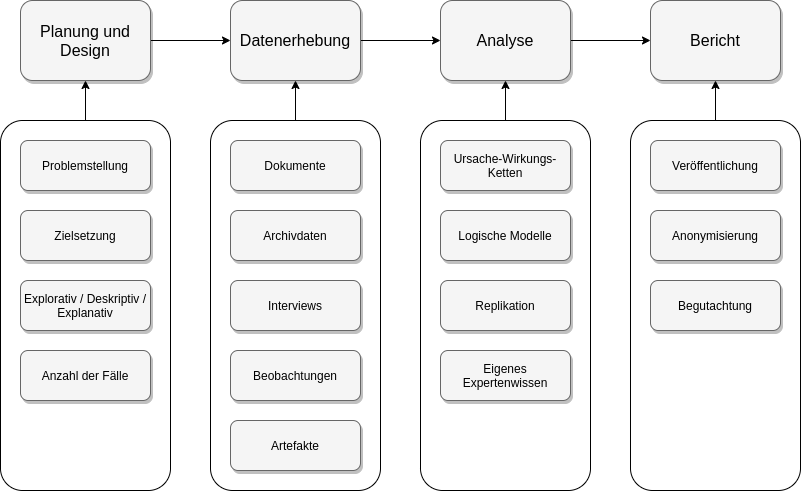
\includegraphics[width=0.8\textwidth]{casestudydesign}
    \label{figure:casestudydesign}
    \\
    \cite[Source: Based on][pp. 8]{gothlich2003fallstudien}
\end{figure}

In the following, the individual steps are described and thereby the design is
defined:\footcite[Cf.][pp. 8]{gothlich2003fallstudien}
\begin{itemize}
    \item \textbf{Planning and design: }The first step is to state the problem and the objectives to be covered by the case study.
    The problem statement is already described in chapter \ref{toc:motivation} and \ref{toc:hypothesenundabgrenzungderarbeit}.
    The goal of this case study is to answer the hypotheses in chapter \ref{toc:ansatzmoeglichkeitenfuerbusinessintelligence}
    by examining its operational feasibility. It is to be increased the resilience of the statements of this work, in that
    planning an application in practice on the basis of the theoretical analysis.
    Therefore, the research objective in the study is exploratory in nature.\footcite[Cf.][p. 8]{gothlich2003fallstudien}
    This case study is conducted once in this form ("single case"). This eliminates any possible replication of this study.\footcite[Cf.][pp. 8]{gothlich2003fallstudien}
    \item \textbf{Data collection: }This step defines the data sources available for the case study. In addition to the
    data sources described in chapter \ref{toc:klassifizierungderdaten}, additional internal documents of the Genesis
    Group are available. These can be found in the appendix to this thesis. Therefore, the case study is based on documents and artifacts.\footcite[Cf.][Table 1 ]{gothlich2003fallstudien}
    \item \textbf{Analysis: }In the course of the analysis, a model for an exemplary \ac{BI} Process,
    which can be applied within the Genesis Group, will be created. On the basis of this it is examined whether the introduction is possible and thereby the
    hypotheses of this thesis can be supported. For this purpose, "cause-effect chains" and logical models are used.\footcite[Cf.][p. 11]{gothlich2003fallstudien}
    In both of these analytical models, strong reference is made to an operational environment.
    \item \textbf{Report: }The final step deals with the publication of this case study. Since this case study takes place in the context
    of this thesis, a publication is already planned. A peer review is nevertheless useful and will be done in the course of
    of the subsequent internal evaluation.
\end{itemize}

In the following, a stakeholder analysis is performed using the Genesis Group as an example. With the help of the results of this analysis and the additional
theoretical knowledge from this thesis, an exemplary \ac{BI} process will be created in chapter \ref{toc:planungdesbiprozesses} and will
finally be checked for its feasibility in chapter \ref{toc:abschliessendebewertung}.

\subsection{Stakeholder analysis for an internal business intelligence process} \label{toc:stakeholderanalyse}

The following stakeholder analysis is primarily based on the publication "A Stakeholder Model of Business
Intelligence" by Claire A. Simmers.\footcite[Cf.][]{simmers2004stakeholder} This work deals with
stakeholder analysis in the field of \ac{BI} and is used for the present analysis. Based on
Figure 14.2 in this publication, the stakeholder analysis is operated and thus the individual persons or groups are identified,
who have an interest in the successful implementation of a \ac{BI} Process.\footcite[Cf.][Fig. 14.2]{simmers2004stakeholder}

The following stakeholders can be identified for cryptomining data center optimization in the cloud mining environment:\footcite[Cf.][Fig. 14.2]{simmers2004stakeholder}\footcite[Cf.][p. 52]{reed2009s}

\begin{itemize}
    \item \textbf{Company owners: }The owners of Genesis Group are responsible for the strategic decisions and
    have an interest in the successful implementation
    of such a \ac{BI} Process. This may include reasons such as improving mining revenue, advantages in the cloud mining market
    through increased data center efficiency, and decision support regarding the new or expansion of mining
    data centers. Therefore, \ac{HT0.1} and \ac{HT0.3} are mainly relevant to these individuals.
    \item \textbf{Employees: }Another relevant group are the employees of the Genesis Group. These benefit
    by the introduction of \ac{BI} especially with regard to time savings, process optimization and
    decision support (Cf. chapter \ref{toc:strategischermehrwert}). This group can be divided into the following subgroups:
    \begin{itemize}
        \item Business management: This group has significant interest in the decision support that a \ac{BI} Process
        provides. Tactical decisions that affect data center operations are made by this group.
        For this reason, management has an interest in an accurate representation of a data center's cash flow, which is
        is reviewed in \ac{HT0.3}.
        \item Management of the data centers: This group manages the existing data centers and can be found in the area of operational decisions.
        It has an interest in operating the most efficient hardware possible (\ac{HT0.2}),
        the cash flow of a data center (\ac{HT0.3}) and the optimization of the staffing of a mining data center
        (\ac{HT0.4}).
        \item Controlling: The controlling department is responsible for the financial monitoring of the data centers. Therefore, this
        group of people has direct interest in a fast and correct access to the financial data from which
        ultimately the cash flow can be calculated (\ac{HT0.3}).
        \item IT: The technical departments are primarily responsible for maintaining and operating the existing hardware.
        Therefore, they mainly need technical \acp{KPI}, which is covered by \ac{HT0.2}. Due to the availability
        of this data, the efficiency of the hardware can be better estimated and possible improvements identified.
    \end{itemize}
    \item \textbf{Investors: }Investors are interested in data, facts, and predictions that are
    are comprehensible and transparent. For these reasons, the group of investors is also one of the stakeholders in a \ac{BI} process,
    since it fulfills exactly these requirements of these stakeholders for an investment object.
    \item \textbf{Suppliers: }Suppliers, such as hardware suppliers or energy providers, are stakeholders of an
    \ac{BI} Process. Their available data is used in such a process, among other things, to optimize the company's purchasing activities.
    By means of \ac{BI}, it is possible, for example, to identify the appropriate hardware for a mining data center
    or to support the selection of the energy supplier.
    \item \textbf{Customers: }Furthermore, the customers who have a cloud mining contract with Genesis Group are stakeholders. These
    have an interest, analogous to the company owners, in obtaining the highest possible and at the same time stable revenue from mining. 
    Therefore, this group has an interest in using the best possible hardware, software and mining pools.
\end{itemize}

The relavant stakeholders from the analysis are summarized visualized in Figure \ref{figure:internalstakeholder}.

\begin{figure}[H]
    \caption{Stakeholders and their main interest in an internal \ac{BI} process}
    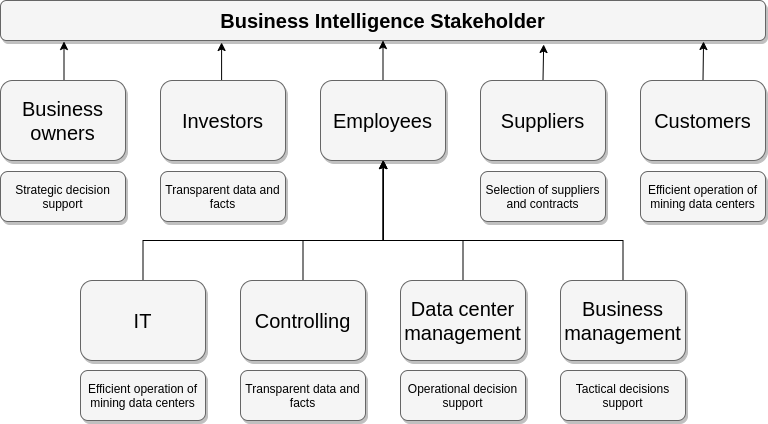
\includegraphics[width=0.8\textwidth]{internalstakeholder}
    \label{figure:internalstakeholder}
\end{figure}

Other groups of stakeholders exist but have no influence on the \ac{BI} evaluation.
These include political groups, governments, and the community.\footcite[Cf.][Fig. 14.2]{simmers2004stakeholder}

\subsection{Planning of the Business Intelligence process} \label{toc:planungdesbiprozesses}

In the following part, an exemplary \ac{BI} Process in an operational environment is planned. The company for which this process is
is planned is the Genesis Group and has already been described in chapter \ref{toc:motivation}. For the planning
the conclusions from chapter \ref{toc:ansatzmoeglichkeitenfuerbusinessintelligence} are used. Within the Genesis Group
the Google Cloud is used for the IT infrastructure, which is why suitable sample products from this cloud are identified in the following
chapters.\footcite[Cf.][]{googlecloud2021dw} Analogous to a \ac{BI} Process, the following study is divided into the steps of data acquisition
(chapter \ref{toc:datenhaltung}), data analysis (chapter \ref{toc:datenanalyse}), and data presentation (chapter \ref{toc:datenpraesentation}).
At the end, there is an evaluation of the study, which includes the argumentation of the sub-hypotheses from chapter
\ref{toc:ansatzmoeglichkeitenfuerbusinessintelligence} and supplements it if necessary.


\subsubsection{Data acquisition} \label{toc:datenhaltung}

Als Datenquellen werden die in Kapitel \ref{toc:klassifizierungderdaten} aufgezeigten Schnittstellen und Systeme verwendet.
Wie aus Tabelle \ref{tbl:klassifizierunginternedaten} und \ref{tbl:klassifizierungexternedaten} hervorgeht, sind alle Datenquellen für die
Verwendung innerhalb eines \ac{BI} geeignet und können daher in dementsprechenden \ac{ETL} Pipelines verwendet werden.
Eine Möglichkeit \ac{ETL} Pipelines in der Cloud errichten zu können, ist die Verwendung des "`Cloud Data Fusion"'
Dienstes.\footcite[Cf.][]{googlecloud2021dw} Dieser ist auf den Aufbau solcher Pipelines spezialisiert und bietet zudem Schnittstellen
zu einem Data Warehouse in der Cloud an. Das Data Warehouse an sich wird über den "`Big Query"' Dienst realisiert.\footcite[Cf.][]{googlecloud2021dw}
Dieses Warehouse ist der zentrale Ort, an dem alle relevanten Daten für die Analysephase des \ac{BI} Prozesses gespeichert werden und
ist daher zusammen mit den \ac{ETL} Pipelines für den Aufbau von \ac{BI} nicht wegzudenken.\footcite[Cf.][pp. 105]{loshin2012business}
Das Data Warehouse wird über den "`Cloud Data Fusion"' Dienst befüllt. Nach diesem Schritt sind alle benötigten Daten intern
im eigenen Data Warehouse verfügbar. Deshalb ist anzunehmen,
dass die Erhebung und die Beschaffung von Daten unter Zuhilfenahme der Google Cloud möglich ist und die betriebliche
Umsetzung für diesen Schritt gegeben ist.

The interfaces and systems shown in chapter \ref{toc:klassifizierungderdaten} are used as data sources.
As shown in table \ref{tbl:klassifizierunginternedaten} and \ref{tbl:klassifizierungexternedaten}, all data sources are suitable for the
use within \ac{BI} and can therefore be used in corresponding \ac{ETL} pipelines.
One way to build \ac{ETL} pipelines in the cloud is to use the "Data Fusion"
service.\footcite[Cf.][]{googlecloud2021dw} This specializes in setting up such pipelines and also provides interfaces
to a data warehouse in the cloud. The data warehouse itself is realized via the "Big Query" service.\footcite[Cf.][]{googlecloud2021dw}
This warehouse is the central location where all relevant data for the analysis phase of the \ac{BI} process is stored and
is therefore indispensable together with the \ac{ETL} pipelines for building a \ac{BI} process.\footcite[Cf.][pp. 105]{loshin2012business}
The data warehouse is populated via the "Cloud Data Fusion" service. After this step, all required data is available internally
in the own data warehouse. Therefore, it can be assumed
that the collection and the acquisition of data with the help of the Google Cloud is possible and that the operational implementation for this step is given.

\subsubsection{Data analysis} \label{toc:datenanalyse}

For the analysis of the data, which is now available in a data warehouse, the analysis procedures are used, which are described in
chapter \ref{toc:analyseverfahrenbi}. In the Google Cloud, there are several possible products for the realization of these procedures.\footcite[Cf.][]{googlecloud2021dw}
These include the products "Looker", which is a \ac{OLAP} platform for \ac{BI},
the "Dataflow" service, which analyzes datasets in real time as well as in batches, and "Dataproc", which has the ability
among other things, to run Apache Spark.\footcite[Cf.][]{googlecloud2021dw} All of these tools are sufficient to complete the analysis phase
of a \ac{BI} process. 

The result from chapter \ref{toc:zusammenfassendebetrachtung} was that the implementation of a \ac{BI} process is possible, but there are
difficulties in predicting the Bitcoin exchange rate. This problem is not directly limited to Bitcoin
itself, but is the case for predicting any exchange rate. 
One way to work with predictive models is not to predict a concrete
price, but to build different scenarios that include possible reactions and decisions of the management.\footcite[Cf.][]{appendix:mcpreis}
An appropriate way to do this is to use stochastic models, especially Monte Carlo simulations.\footcite[Cf.][p. 28]{cocco2016modeling}
These are already used for scenario building in the Genesis Group. The Monte Carlo simulation at hand was
made on 06.11.2020.\footcite[Cf.][]{appendix:mcpreis} When comparing to real data from this time, it is noticeable that this form of simulation is suitable
for predictive models for the near future (< 1 month).\footcite[Cf.][]{appendix:btcusd} The further events were largely determined by social media
and therefore could not be mapped within the scope of this simulation.
This form of simulation gives the possibility
to calculate and statistically evaluate any number of possible price developments.
evaluation.\footcite[Cf.][]{appendix:mcpreis}\footcite[Cf.][]{appendix:mcszenarien} This results in multiple
scenarios that imply different management responses. The initial values for such an analysis
are provided by the data warehouse. The results
are in turn entered into the data warehouse and are thus accessible to other analysis procedures. However, as already
in chapter \ref{toc:ansatzmoeglichkeitenfuerbusinessintelligence}, social media platforms, for example, have a major influence on the
development of the Bitcoin price. Such developments cannot be represented directly with stochastic models.
Here again, real-time processing of the data is important so that the stakeholders already described can react directly.
In addition to the development of the Bitcoin price, it is possible through a Monte-Carlo simulation to show the development of the entire
network hashrate of the Bitcoin network.\footcite[Cf.][]{appendix:mchashrate}

It can be seen that by switching from strict predictive models to coarser scenario building,
the predictive aspect of \ac{BI} can be implemented. Also, for sub-hypotheses one and three, predictive and
prescriptive \ac{BI} is possible. Operational feasibility is given.

\subsubsection{Data presentation} \label{toc:datenpraesentation}

This part deals with the process of how the knowledge generated by the appropriate analysis of the data is now made available to the
relevant stakeholders in the correct manner, thereby achieving the goal of decision support.
For this purpose, the stakeholders from chapter \ref{toc:stakeholderanalyse} are considered in the following. There are several
ways in which knowledge can be made available to these individuals and groups:\footcite[Cf.][Chap. 19]{loshin2012business}
\begin{itemize}
    \item \textbf{Reporting: }This is the simplest form of presentation. In this case
    static report templates are configured, from which regular reports are automatically generated and made available to the stakeholders.\footcite[Cf.][p. 305]{loshin2012business}
    Examples of such reports in the context of this work include reports on mining downtime
    or monthly summaries of the financial situation of data centers. The generation of such reports can be done in
    Google Cloud via the "Cloud Scheduler".\footcite[Cf.][]{googlecloud2021scheduler} The relevant stakeholders can be provided with the reports accordingly.
    \item \textbf{\ac{OLAP} and Ad-Hoc Searches: }In this form of presentation, a \ac{OLAP} system is used to create one's own search queries
    and thus generate tailored knowledge.\footcite[Cf.][pp. 308]{loshin2012business}
    These search queries can be created spontaneously (ad-hoc) through the \ac{OLAP} system
    and results are provided directly to the stakeholder. Examples include queries that concern the new construction or
    expansion of mining data centers. An example of such a system is the "Looker" service of the
    Google Cloud.\footcite[Cf.][]{googlecloud2021dw}
    \item \textbf{Dashboards: }Another method of making analytics knowledge available to stakeholders
    is the use of dashboards. These dashboards
    can be accessed online and present data obtained through the underlying software.\footcite[Cf.][pp. 314]{loshin2012business} Especially for
    technical \acp{KPI}, such as the display of hashrates or power consumption of the hardware, this form of
    visualization is used. Furthermore, stakeholders are able to create their own dashboards.\footcite[Cf.][pp. 314]{loshin2012business}
    A common application for creating dashboards is "Grafana".\footnote{https://grafana.com}
    \item \textbf{Alerting: }This method proactively sends notifications and alerts to
    relevant stakeholders.\footcite[Cf.][pp. 311]{loshin2012business} This enables them to respond to changing circumstances with only a small time lag. For example,
    the complete failure of a data center or deviations of reality from the forecast models are cases in which an alert can make sense.
    Such alerts can then be delivered to the relevant stakeholders via mail or instant messenger.\footcite[Cf.][pp. 311]{loshin2012business}
    A service that allows the creation of such alerts is the "Pub/Sub" service.\footcite[Cf.][]{googlecloud2021dw} For the sending of alerts
    monitoring systems, such as "Prometheus", can be used.\footnote{https://prometheus.io}
\end{itemize}

All these forms of presentation can easily be carried out in-house. Therefore, there are no internal obstacles
to the implementation of an \ac{BI} process.

\subsection{Final evaluation} \label{toc:abschliessendebewertung}

In chapter \ref{toc:planungdesbiprozesses}, a small case study discussed whether it is possible to implement a \ac{BI} Process,
as it was shown in chapter \ref{toc:ansatzmoeglichkeitenfuerbusinessintelligence}.
In order to achieve this, the three main steps of an \ac{BI} process, data acquisition, analysis and presentation, were discussed individually
and possible technical solutions were demonstrated using the Google Cloud as an example.

In summary, it can be stated that there are no obstacles that contradict the introduction of an \ac{BI} process.
In addition to the argumentation from chapter \ref{toc:ansatzmoeglichkeitenfuerbusinessintelligence}, it is possible that the \ac{BI} Process
is feasible up to the prescriptive paradigm (Cf. Table \ref{tbl:hypothesenanalyse2}). Therefore, it is possible without restriction that all sub-hypotheses
can be mapped in such a process. Thus, in conclusion it is possible to say that the main hypothesis of this work can be confirmed.
By means of \ac{BI} it is possible that cryptomining data centers can be optimized financially.

\begin{table}[H]
    \caption{Result of the feasibility of a business intelligence process}
    \label{tbl:hypothesenanalyse2}
    \begin{tabularx}{\textwidth}[ht]{X||c|c|c|c}
         & \ac{HT0.1} & \ac{HT0.2} & \ac{HT0.3} & \ac{HT0.4}  \\
        \hline\hline
        Descriptive analysis & \checkmark & \checkmark & \checkmark & \checkmark \\
        \hline
        Predictive analysis & \checkmark & \checkmark & \checkmark & \checkmark \\
        \hline
        Prescriptive analysis & \checkmark & \checkmark & \checkmark & \checkmark \\
    \end{tabularx}
\end{table}

An example \ac{BI} Process for the Genesis Group example may look like the one shown in Figure \ref{figure:internalbiprocess}.

\begin{figure}[H]
    \caption{Design of a BI process within the Genesis Group}
    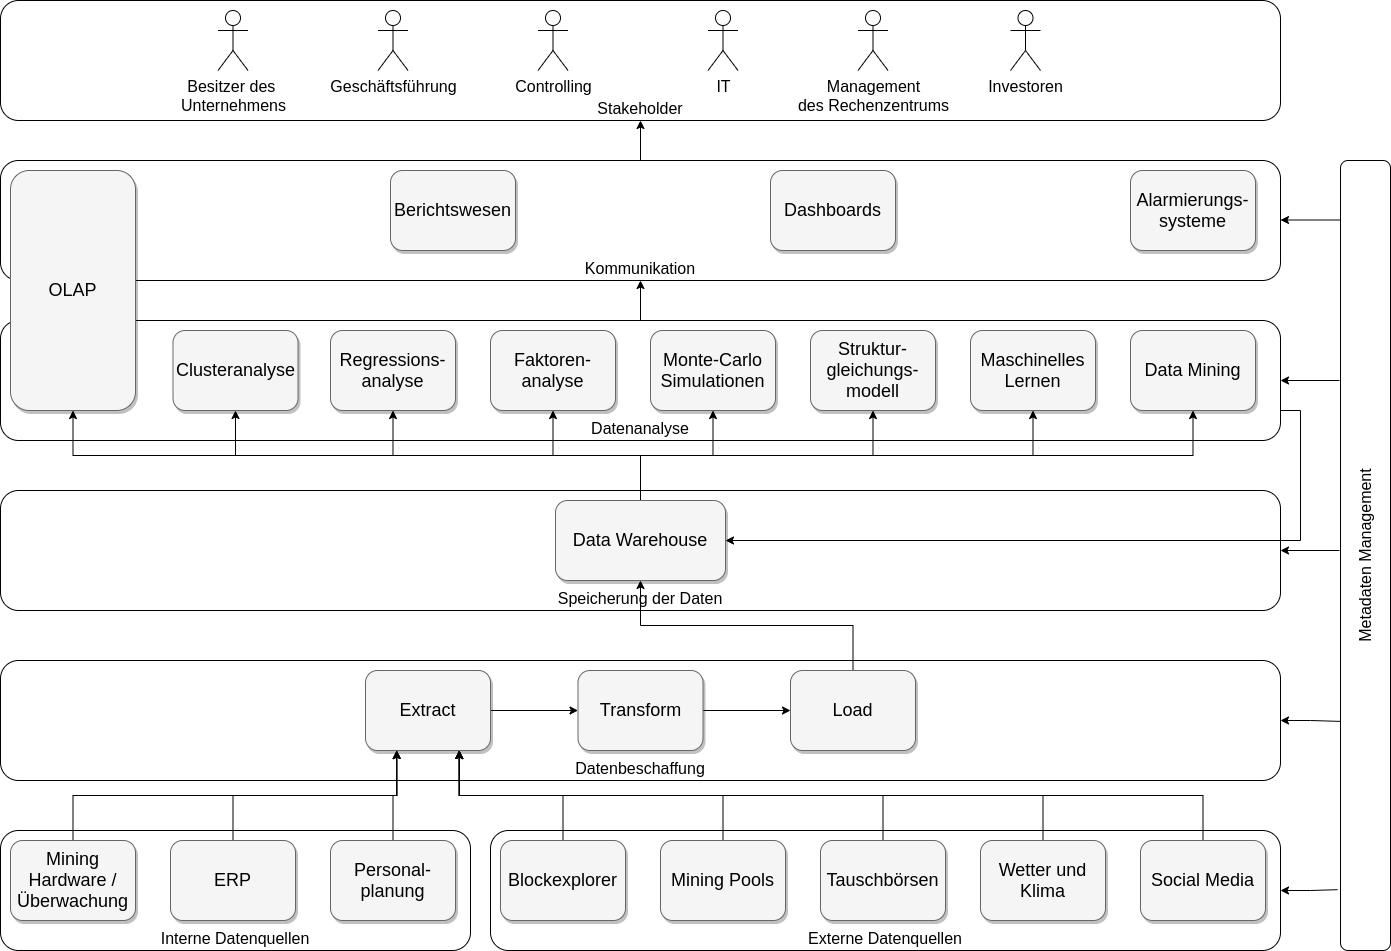
\includegraphics[width=\textwidth]{internalbiprocess}
    \label{figure:internalbiprocess}
\end{figure}

This figure is basically based on the process structure shown in chapter \ref{toc:prozess}, and is divided into the following
steps:
\begin{itemize}
    \item \textbf{Data sources: }The data sources are the services described in chapters \ref{toc:internedatenquellen} and \ref{toc:externedatenquellen}.
    All of these sources together are sufficient to provide enough data to prove the four sub-hypotheses and
    thereby the main hypothesis.
    \item \textbf{Data acquisition: }Data sourcing involves \ac{ETL} pipelines that interrogate data at the interfaces
    to the sources, transform them into the desired format, and ultimately store them in a data warehouse. As
    in the classification of data sources from table \ref{tbl:klassifizierunginternedaten} and \ref{tbl:klassifizierungexternedaten},
    as well as chapter \ref{toc:datenhaltung}, the \ac{ETL} pipelines can be built and realized without any obstacles.
    \item \textbf{Storage of data / data management: }In the third step, the extracted and structured data are loaded into a data warehouse.
    This contains all data that is still important for the \ac{BI} process to be able to present results to the stakeholders.
    This part can be implemented as shown in chapter \ref{toc:datenhaltung}.
    \item \textbf{Data analysis: }The stored data is subsequently used for analysis in order to be able to generate new knowledge.
    There are many different approaches for the analysis of data, which have been discussed in detail in chapter \ref{toc:analyseverfahrenbi}.
    These are used to find out the optimization potential of a cryptomining data center and to identify
    possible approaches for implementation. All of these forms of analysis can be implemented in-house
    without further ado. However, the exact design of the analysis algorithms is a lengthy and complex process
    and will not be discussed in the course of this thesis, since the basic possibility of implementation is discussed in this work.
    \item \textbf{Communication / Presentation: }The final step is to present the data in a manner, 
    through which the stakeholders of the \ac{BI} process can access and further use the knowledge.
    Relevant forms of presentation are described in
    chapter \ref{toc:datenpraesentation} and are sufficient to ensure that stakeholders can be guided in an optimal way through the
    \ac{BI} Process. Implementation of this level is straightforward.
\end{itemize}

In the following chapter, the conclusion from this and the last chapter is subjected to a critical evaluation in order to
finally be able to put the answer to the main hypothesis into the right context.